\documentclass{article}
\usepackage{geometry}
\geometry{a4paper, landscape, margin=1.5cm}
\usepackage{graphicx}
\graphicspath{ {images/} }
\usepackage{listings}
\date{28nd May 2021}
\author{\Large submitted by\\ Arghya Bandyopadhyay\\
    	RollNo. 20CS4103\\}
\title{\begin{center}
       \bfseries\Large
    	Assignment 1\\
    	Of\\
    	Network \& Distributed System Lab (CS2051)\\
        \vskip1cm
        Masters of Technology in Computer Science And Engineering\\
    	\vskip1cm
    	submitted to\\
    	Dr Sujoy Saha\\
    	Assistant Professor\\
    	Dept. of CSE\\
    	\vskip1cm
    	
\includegraphics[width=4cm]{NITDGP}\\
    	National Institute of Technology, Durgapur\\
    \end{center}}
\date{27th March 2021}
\begin{document}
\maketitle
\pagebreak
\begin{enumerate}
\item Write simple TCP and UDP program using socket API which will transfer simple text
messages, and check TCP and UDP packets using Wireshark.
\begin{flushleft}
\textbf{Answer.}
\end{flushleft}

The following code is the implementation for \textbf{TCP client side programming}.
\begin{lstlisting}
	
/* tcpclient.c */

#include <sys/socket.h>
#include <sys/types.h>
#include <netinet/in.h>
#include <netdb.h>
#include <stdio.h>
#include <string.h>
#include <stdlib.h>
#include <unistd.h>
#include <errno.h>


int main()
{

        int sock, bytes_recieved;  
        char send_data[1024],recv_data[1024];
        struct hostent *host;
        struct sockaddr_in server_addr;  

        host = gethostbyname("127.0.0.1");

        if ((sock = socket(AF_INET, SOCK_STREAM, 0)) == -1) {
            perror("Socket");
            exit(1);
        }

        server_addr.sin_family = AF_INET;     
        server_addr.sin_port = htons(5000);   
        server_addr.sin_addr = *((struct in_addr *)host->h_addr);
        bzero(&(server_addr.sin_zero),8); 

        if (connect(sock, (struct sockaddr *)&server_addr,
                    sizeof(struct sockaddr)) == -1) 
        {
            perror("Connect");
            exit(1);
        }

        while(1)
        {
        
          bytes_recieved=recv(sock,recv_data,1024,0);
          recv_data[bytes_recieved] = '\0';
 
          if (strcmp(recv_data , "q") == 0 || strcmp(recv_data , "Q") == 0)
          {
           close(sock);
           break;
          }

          else
           printf("\nRecieved data = %s " , recv_data);
           
           printf("\nSEND (q or Q to quit) : ");
           gets(send_data);
           
          if (strcmp(send_data , "q") != 0 && strcmp(send_data , "Q") != 0)
           send(sock,send_data,strlen(send_data), 0); 

          else
          {
           send(sock,send_data,strlen(send_data), 0);   
           close(sock);
           break;
          }
        
        }   
return 0;
}
\end{lstlisting}

The following code is the implementation for \textbf{TCP Server side programming}.
\begin{lstlisting}

/* tcpserver.c */

#include <sys/types.h>
#include <sys/socket.h>
#include <netinet/in.h>
#include <arpa/inet.h>
#include <stdio.h>
#include <stdlib.h>
#include <unistd.h>
#include <errno.h>
#include <string.h>


int main()
{
        int sock, connected, bytes_recieved , true = 1;  
        char send_data [1024] , recv_data[1024];       

        struct sockaddr_in server_addr,client_addr;    
        int sin_size;
        
        if ((sock = socket(AF_INET, SOCK_STREAM, 0)) == -1) {
            perror("Socket");
            exit(1);
        }

        if (setsockopt(sock,SOL_SOCKET,SO_REUSEADDR,&true,sizeof(int)) == -1) {
            perror("Setsockopt");
            exit(1);
        }
        
        server_addr.sin_family = AF_INET;         
        server_addr.sin_port = htons(5000);     
        server_addr.sin_addr.s_addr = INADDR_ANY; 
        bzero(&(server_addr.sin_zero),8); 

        if (bind(sock, (struct sockaddr *)&server_addr, sizeof(struct sockaddr))
                                                                       == -1) {
            perror("Unable to bind");
            exit(1);
        }

        if (listen(sock, 5) == -1) {
            perror("Listen");
            exit(1);
        }
		
	printf("\nTCPServer Waiting for client on port 5000");
        fflush(stdout);


        while(1)
        {  

            sin_size = sizeof(struct sockaddr_in);

            connected = accept(sock, (struct sockaddr *)&client_addr,&sin_size);

            printf("\n I got a connection from (%s , %d)",
                   inet_ntoa(client_addr.sin_addr),ntohs(client_addr.sin_port));

            while (1)
            {
              printf("\n SEND (q or Q to quit) : ");
              gets(send_data);
              
              if (strcmp(send_data , "q") == 0 || strcmp(send_data , "Q") == 0)
              {
                send(connected, send_data,strlen(send_data), 0); 
                close(connected);
                break;
              }
               
              else
                 send(connected, send_data,strlen(send_data), 0);  

              bytes_recieved = recv(connected,recv_data,1024,0);

              recv_data[bytes_recieved] = '\0';

              if (strcmp(recv_data , "q") == 0 || strcmp(recv_data , "Q") == 0)
              {
                close(connected);
                break;
              }

              else 
              printf("\n RECIEVED DATA = %s " , recv_data);
              fflush(stdout);
            }
        }       

      close(sock);
      return 0;
} 
\end{lstlisting}

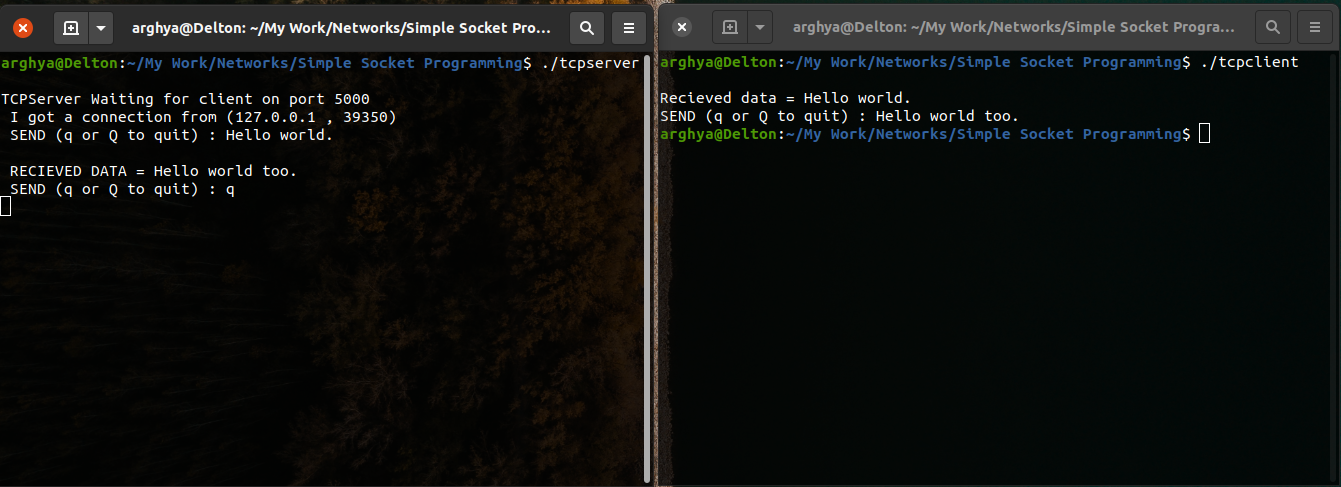
\includegraphics[width=700pt]{Question11}

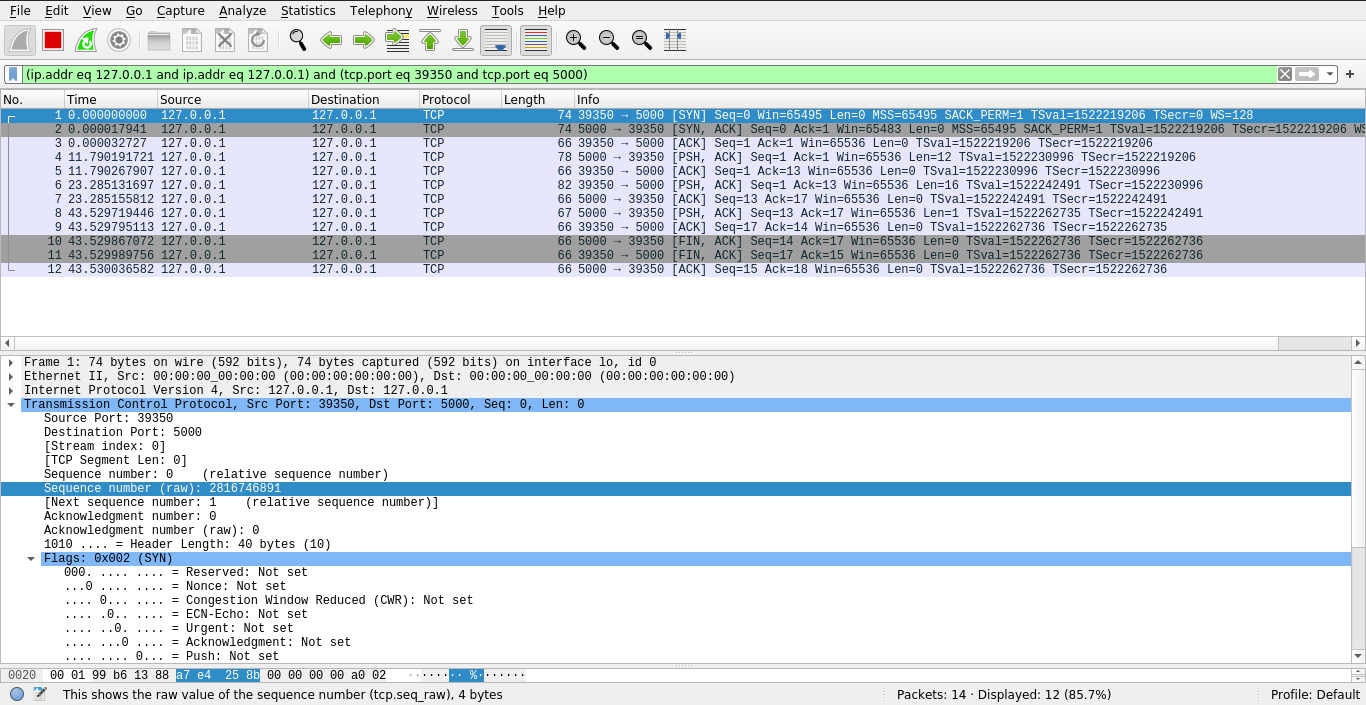
\includegraphics[width=700pt]{Question12}
\pagebreak

The following code is the implementation for \textbf{UDP Client side programming}.
\begin{lstlisting}

/* udpclient.c */ 

#include <sys/types.h>
#include <sys/socket.h>
#include <netinet/in.h>
#include <arpa/inet.h>
#include <netdb.h>
#include <stdio.h>
#include <unistd.h>
#include <errno.h>
#include <string.h>
#include <stdlib.h>

int main()
{
	int sock;
	struct sockaddr_in server_addr;
	struct hostent *host;
	char send_data[1024];

	host= (struct hostent *) gethostbyname((char *)"127.0.0.1");


if ((sock = socket(AF_INET, SOCK_DGRAM, 0)) == -1)
{
	perror("socket");
	exit(1);
}

	server_addr.sin_family = AF_INET;
	server_addr.sin_port = htons(5000);
	server_addr.sin_addr = *((struct in_addr *)host->h_addr);
	bzero(&(server_addr.sin_zero),8);

   while (1)
   {

	    printf("Type Something (q or Q to quit):");
	    gets(send_data);

 	   if ((strcmp(send_data , "q") == 0) || strcmp(send_data , "Q") == 0)
     	  break;

    	else
       		sendto(sock, send_data, strlen(send_data), 0,
              	(struct sockaddr *)&server_addr, sizeof(struct sockaddr));
     
   }

}

\end{lstlisting}

The following code is the implementation for \textbf{UDP Server side programming}.
\begin{lstlisting}

/* udpserver.c */ 

#include <sys/types.h>
#include <sys/socket.h>
#include <netinet/in.h>
#include <arpa/inet.h>
#include <stdio.h>
#include <unistd.h>
#include <errno.h>
#include <string.h>
#include <stdlib.h>

int main()
{
        int sock;
        int addr_len, bytes_read;
        char recv_data[1024];
        struct sockaddr_in server_addr , client_addr;


        if ((sock = socket(AF_INET, SOCK_DGRAM, 0)) == -1) {
            perror("Socket");
            exit(1);
        }

        server_addr.sin_family = AF_INET;
        server_addr.sin_port = htons(5000);
        server_addr.sin_addr.s_addr = INADDR_ANY;
        bzero(&(server_addr.sin_zero),8);


        if (bind(sock,(struct sockaddr *)&server_addr,
            sizeof(struct sockaddr)) == -1)
        {
            perror("Bind");
            exit(1);
        }

        addr_len = sizeof(struct sockaddr);
		
	printf("\nUDPServer Waiting for client on port 5000");
        fflush(stdout);

	while (1)
	{

          bytes_read = recvfrom(sock,recv_data,1024,0,
	                    (struct sockaddr *)&client_addr, &addr_len);
	  

	  recv_data[bytes_read] = '\0';

          printf("\n(%s , %d) said : ",inet_ntoa(client_addr.sin_addr),
                                       ntohs(client_addr.sin_port));
          printf("%s", recv_data);
	  fflush(stdout);

        }
        return 0;
}

\end{lstlisting}

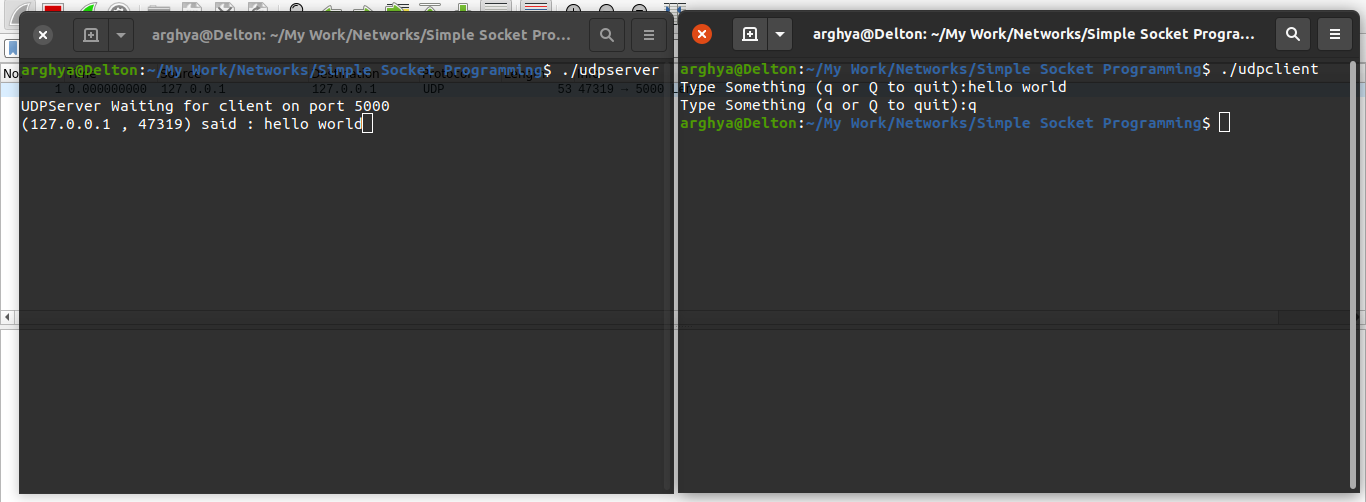
\includegraphics[width=700pt]{Question13}

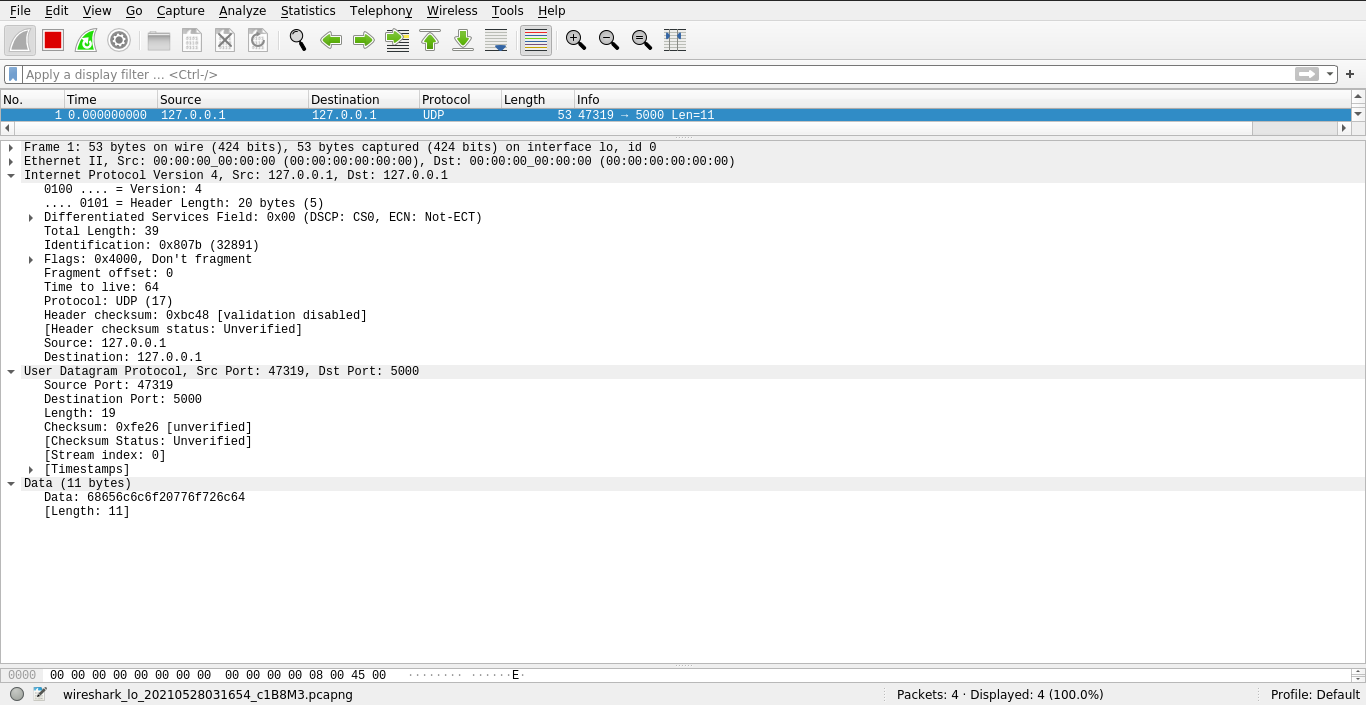
\includegraphics[width=700pt]{Question14}

\pagebreak
\item Using wireshark, capture the TCP headers while connecting your computer to the
server of nit.dgp.ac.in.
\begin{flushleft}
\textbf{Answer.}

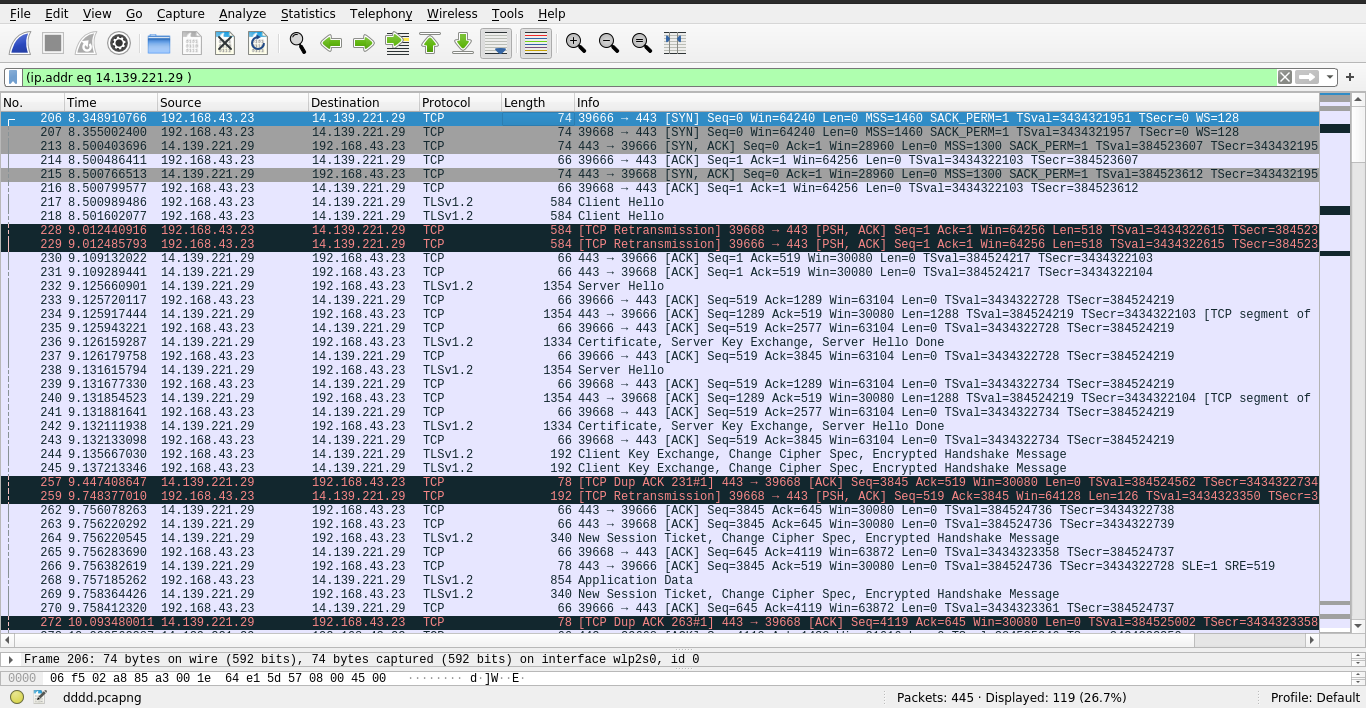
\includegraphics[width=700pt]{Question21}
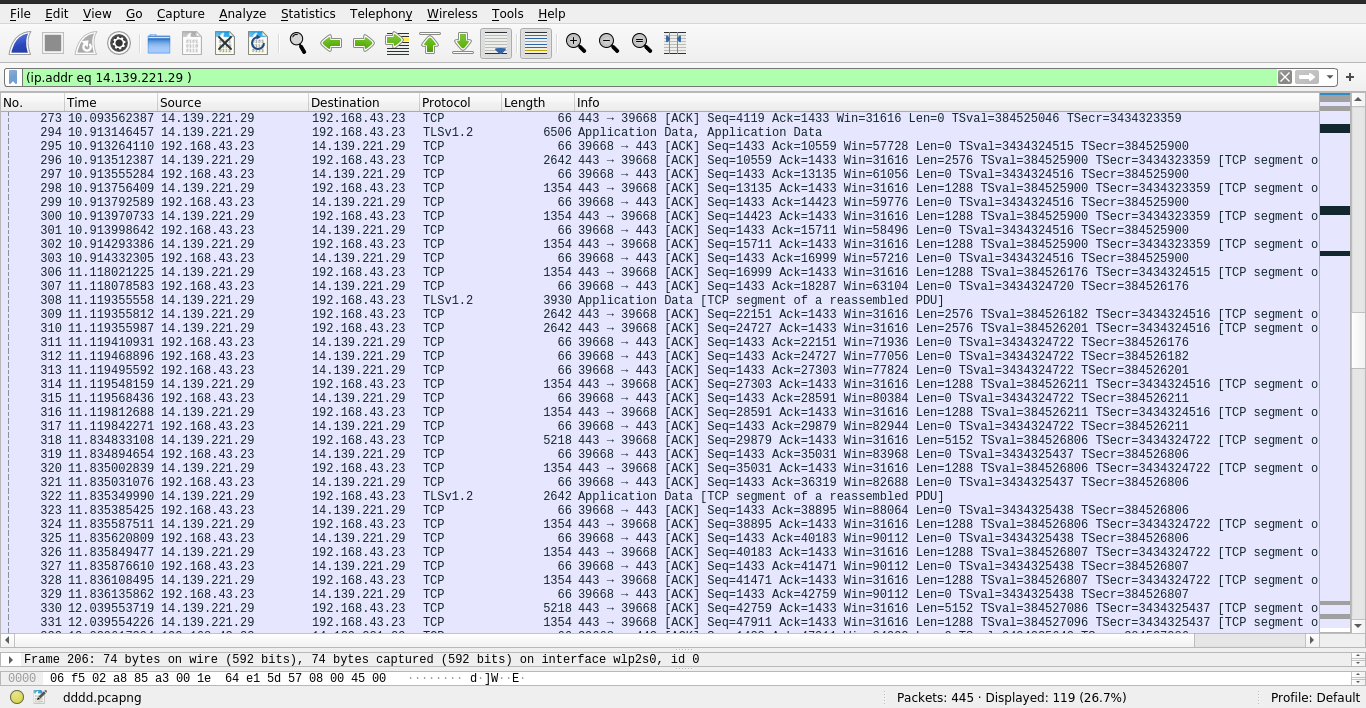
\includegraphics[width=700pt]{Question22}
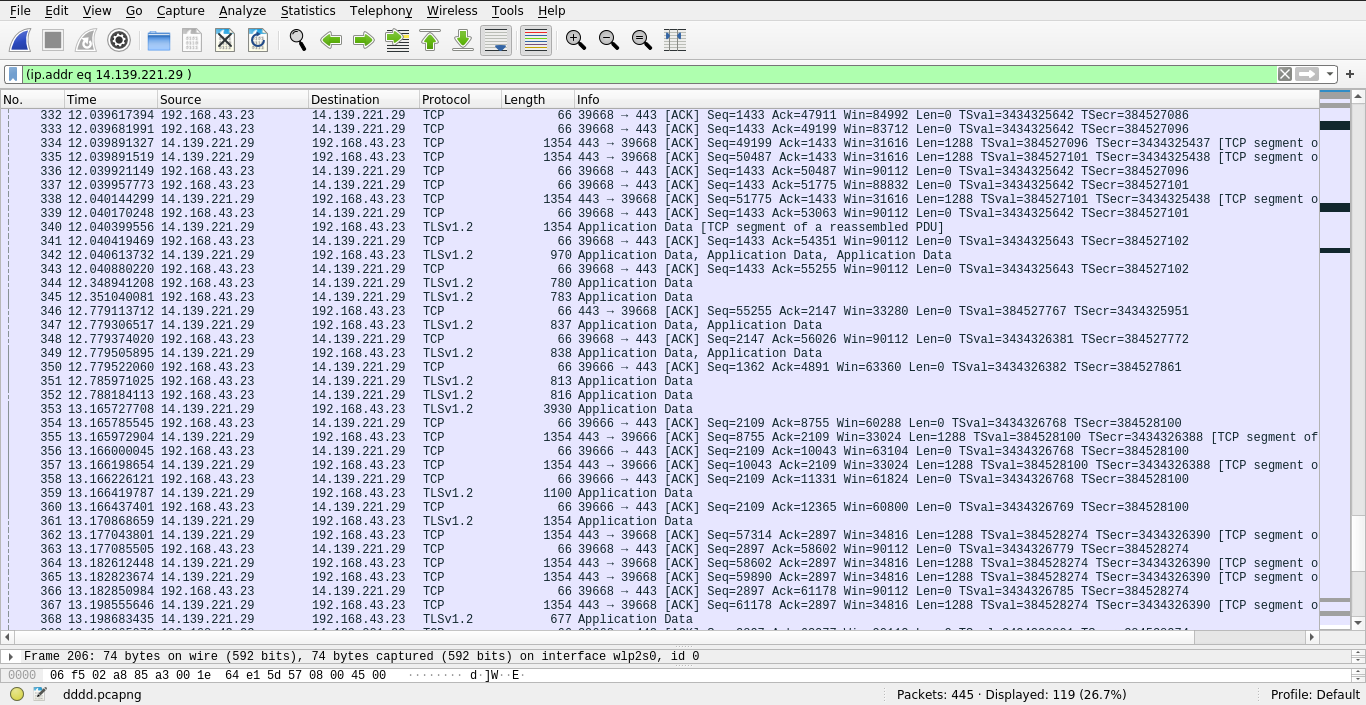
\includegraphics[width=700pt]{Question23}
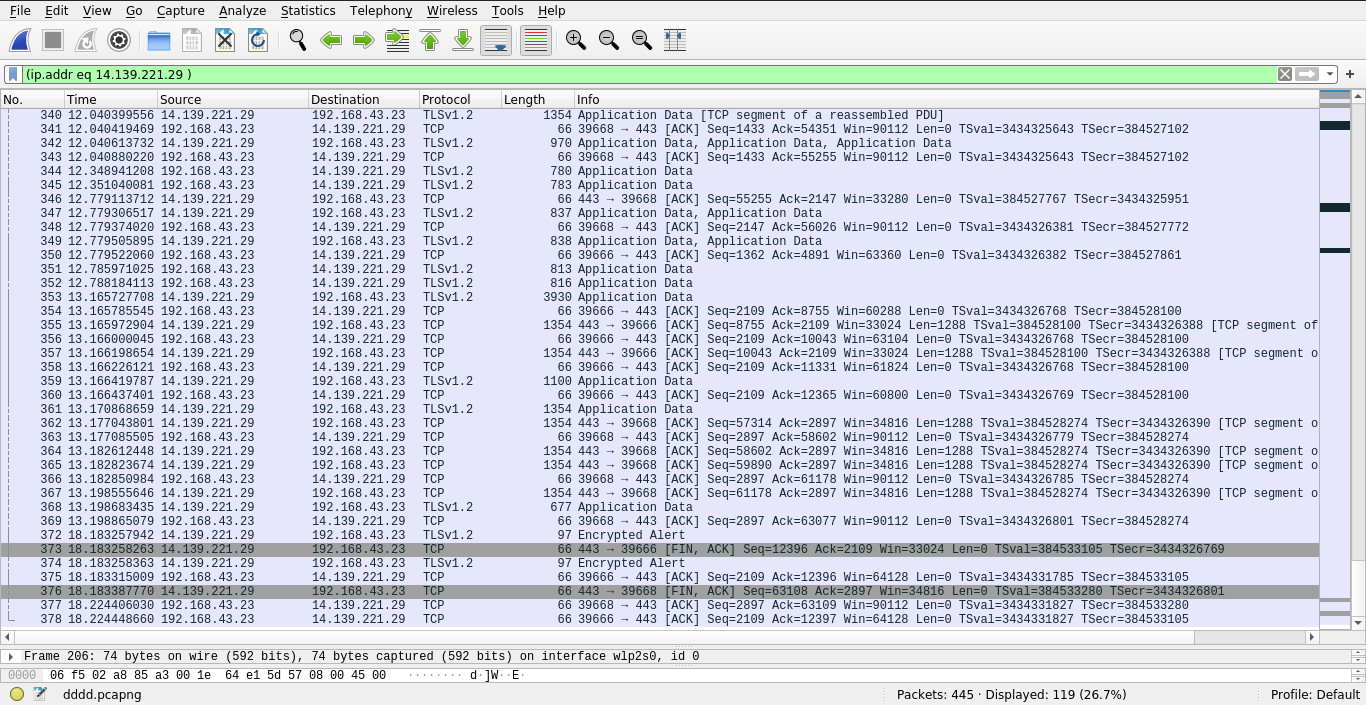
\includegraphics[width=700pt]{Question24}
\end{flushleft}
\pagebreak
\item \begin{enumerate}
\item Show how the six flags (SYN, ACK, PUSH, URGENT, RST, FIN) are working in TCP protocol

\textbf{Answer.}

\item What is the IP address of nitdgp.ac.in? On what port number is it sending and receiving
TCP segments for this connection?

\textbf{Answer.} The IP address of nitdgp.ac.in is \textbf{14.139.221.29} and the tcp port number for sending and receiving TCP segments for the connections are \textbf{443} respectively.

\item Write a small socket program for the URGENT pointer and urgent flag?

\textbf{Answer.}

\begin{lstlisting}

/* bindacpt.h */ 

#include <stdio.h>
#include <unistd.h>
#include <stdlib.h>
#include <errno.h>
#include <string.h>
#include <signal.h>
#include <fcntl.h>
#include <sys/types.h>
#include <sys/socket.h>
#include <netinet/in.h>
#include <arpa/inet.h>
#include <netdb.h>
#include <ctype.h>

int confd;
int mkaddr(void *addr,  
		int *addrlen,  
		char *str_addr,  
		char *protocol) {  

	char *inp_addr = strdup(str_addr);  
	char *host_part = strtok(inp_addr, ":" );  
	char *port_part = strtok(NULL, "\n" );  
	struct sockaddr_in *ap =  
		(struct sockaddr_in *) addr;  
	struct hostent *hp = NULL;  
	struct servent *sp = NULL;  
	char *cp;  
	long lv;  

	/* 
	 * Set input defaults: 
	 */  
	if ( !host_part ) {  
		host_part =  "*" ;  
	}  
	if ( !port_part ) {  
		port_part =  "*" ;  
	}  
	if ( !protocol ) {  
		protocol =  "tcp" ;  
	}  

	/* 
	 * Initialize the address structure: 
	 */  
	memset(ap,0,*addrlen);  
	ap->sin_family = AF_INET;  
	ap->sin_port = 0;  
	ap->sin_addr.s_addr = INADDR_ANY;  

	/* 
	 * Fill in the host address: 
	 */  
	if ( strcmp(host_part, "*" ) == 0 ) {  
		; /* Leave as INADDR_ANY */  
	}  
	else if ( isdigit(*host_part) ) {  
		/* 
		 * Numeric IP address: 
		 */  
		ap->sin_addr.s_addr =  
			inet_addr(host_part);  
		// if ( ap->sin_addr.s_addr == INADDR_NONE ) {  
		if ( !inet_aton(host_part,&ap->sin_addr) ) {  
			return -1;  
		}  
	}   
		else {  
			/* 
			 * Assume a hostname: 
			 */  
			hp = gethostbyname(host_part);  
			if ( !hp ) {  
				return -1;  
			}  
			if ( hp->h_addrtype != AF_INET ) {  
				return -1;  
			}  
			ap->sin_addr = * (struct in_addr *)  
				hp->h_addr_list[0];  
		}  

		/* 
		 * Process an optional port #: 
		 */  
		if ( !strcmp(port_part, "*" ) ) {  
			/* Leave as wild (zero) */  
		}  
		else if ( isdigit(*port_part) ) {  
			/* 
			 * Process numeric port #: 
			 */  
			lv = strtol(port_part,&cp,10);  
			if ( cp != NULL && *cp ) {  
				return -2;  
			}  
			if ( lv < 0L || lv >= 32768 ) {  
				return -2;  
			}  
			ap->sin_port = htons( (short)lv);  
		}   
		else {  
			/* 
			 * Lookup the service: 
			 */  
			sp = getservbyname( port_part, protocol);  
			if ( !sp ) {  
				return -2;  
			}  
			ap->sin_port = (short) sp->s_port;  
		}  

		/*  
		 * Return address length  
		 */  
		*addrlen = sizeof *ap;  

		free(inp_addr);  
		return 0;  
	}  

void sigurg(int signo)
{
	char buf[256];
	int	n;
	printf("SIGURG received \n");
	n = recv(confd, buf, sizeof(buf)-1, MSG_OOB);
	buf[n] = 0;
	fprintf(stdout, "read %d OOB bytes :%s\n", n, buf);
}

void  bail(const char *on_what) {
      if ( errno != 0 ) {
          fputs(strerror(errno),stderr);
          fputs(": ",stderr);
      }
      fputs(on_what,stderr);
      fputc('\n',stderr);
      exit(1);
  }

int  BindAccept(char *addr) {
      int z;
      int s;
      struct sockaddr_in adr_srvr;
      struct sockaddr_in adr_clnt;
      int len_inet;

      /*
      * Create a TCP/IP socket to use:
       */
      s = socket(PF_INET,SOCK_STREAM,0);
      if ( s == -1 )
          bail("socket()");

      /*
       * Bind the server address:
       */
      len_inet = sizeof adr_srvr;
      z = mkaddr(&adr_srvr,&len_inet,
      addr,"tcp");

      if ( z != 0 ) {
          puts("Bad address/port");
          exit(1);
      }

      /*
       * Bind server address:
       */
      z = bind(s,(struct sockaddr *)&adr_srvr,
             len_inet);
      if ( z == -1 )
          bail("bind(2)");

      /*
       * Set listen mode:
       */
      if ( listen(s,10) == -1 )
          bail("listen(2)");

      /*
       * Wait for a connect:
       */
      len_inet = sizeof adr_clnt;

      z = accept(s,
          (struct sockaddr *)&adr_clnt,
          &len_inet);

      if ( z == -1 )
              bail("accept(2)");

      close(s);   /* No longer needed */
      return z;   /* Connected socket */
  }
int Connect(char *addr) {
     int z;
     int s;
     struct sockaddr_in adr_srvr;
     int len_inet;
     /*
      * Create a TDP/IP socket to use:
      */
     s = socket(PF_INET,SOCK_STREAM,0);
     if ( s == -1 )
         bail("socket()");

     /*
      * Bind the server address:
      */
     len_inet = sizeof adr_srvr;
     z = mkaddr(&adr_srvr,&len_inet,
         addr,"tcp");

     if ( z != 0 ) {
        puts("Bad address/port");
         exit(1);
     }

     /*
      * Connect to server:
      */
     len_inet = sizeof adr_srvr;

     z = connect(s,
         (struct sockaddr *)&adr_srvr,
         len_inet);

     if ( z == -1 )
             bail("connect(2)");

     return s;   /* Connected socket */
 }

\end{lstlisting}

\begin{lstlisting}

/* tcpclient01.c */ 

#include "bindacpt.h"
#include <stdio.h>
#include <unistd.h>
#include <stdlib.h>
#include <errno.h>
#include <string.h>
#include <signal.h>
#include <fcntl.h>
#include <sys/types.h>
#include <sys/socket.h>
#include <netinet/in.h>
#include <arpa/inet.h>
#include <netdb.h>
#include <ctype.h>  

static void iband(int s,char *str) {
      int z;

      z = send(s,str,strlen(str),0);
      if ( z == -1 )
          bail("send(2)");

      printf("ib: '%s' (%d)\n",str,z);
  }

  /*
   * Send out-of-band data:
   */
  static void
  oband(int s,char *str) {
      int z;

      z = send(s,str,strlen(str),MSG_OOB);
      if ( z == -1 )
          bail("send(2)");

     printf("OOB '%s' (%d)\n",str,z);
  }

  int
  main(int argc,char **argv) {
      int s = -1;      /* Socket */

      s = Connect(argc >= 2
          ? argv[1]
          : "127.0.0.1:9011");

      iband(s,"In the beginning");
      sleep(1);
      iband(s,"Linus begat Linux,");
      sleep(1);

      iband(s,"and the Penguins");
      sleep(1);

      oband(s,"rejoiced");
      sleep(1);

      iband(s,"exceedingly.");
      close(s);

      return 0;
  }

\end{lstlisting}

\begin{lstlisting}

/* tcpserver01.c */ 

#include "bindacpt.h"
#include <stdio.h>
#include <unistd.h>
#include <stdlib.h>
#include <errno.h>
#include <string.h>
#include <signal.h>
#include <fcntl.h>
#include <sys/types.h>
#include <sys/socket.h>
#include <netinet/in.h>
#include <arpa/inet.h>
#include <netdb.h>
#include <ctype.h>  

int listenfd;

int	main(int argc, char **argv)
{
	int	n;
	int z;
	char buf[256];
	listenfd = BindAccept(argc >= 2? argv[1]: "127.0.0.1:9011");
	z = fcntl(listenfd,F_SETOWN,getpid());
	if ( z == -1 ) bail("fcntl(2)");
	signal(SIGURG,sigurg);
	for (;;) {
          z = recv(listenfd,buf,sizeof buf,0);
          if ( z == -1 )
              bail("recv(2)");
          if ( z == 0 )
              break;
          buf[z] = 0;

          printf("rcv '%s' (%d)\n",
              buf, z);
     }
	  close(listenfd);
	  return 0;
	exit(0);
}

\end{lstlisting}
\pagebreak
\item What is the sequence number of the TCP SYN segment that is used to initiate the TCP
connection between the client computer and nitdgp.ac.in?

\textbf{Answer.} Relative sequence number is 0. And actual sequence number is \textbf{3520860541}. The sequence number	of the TCP SYN segment is 0	since it is used to initate	the	TCP	connection between the client computer and	nitdgp.ac.in.	

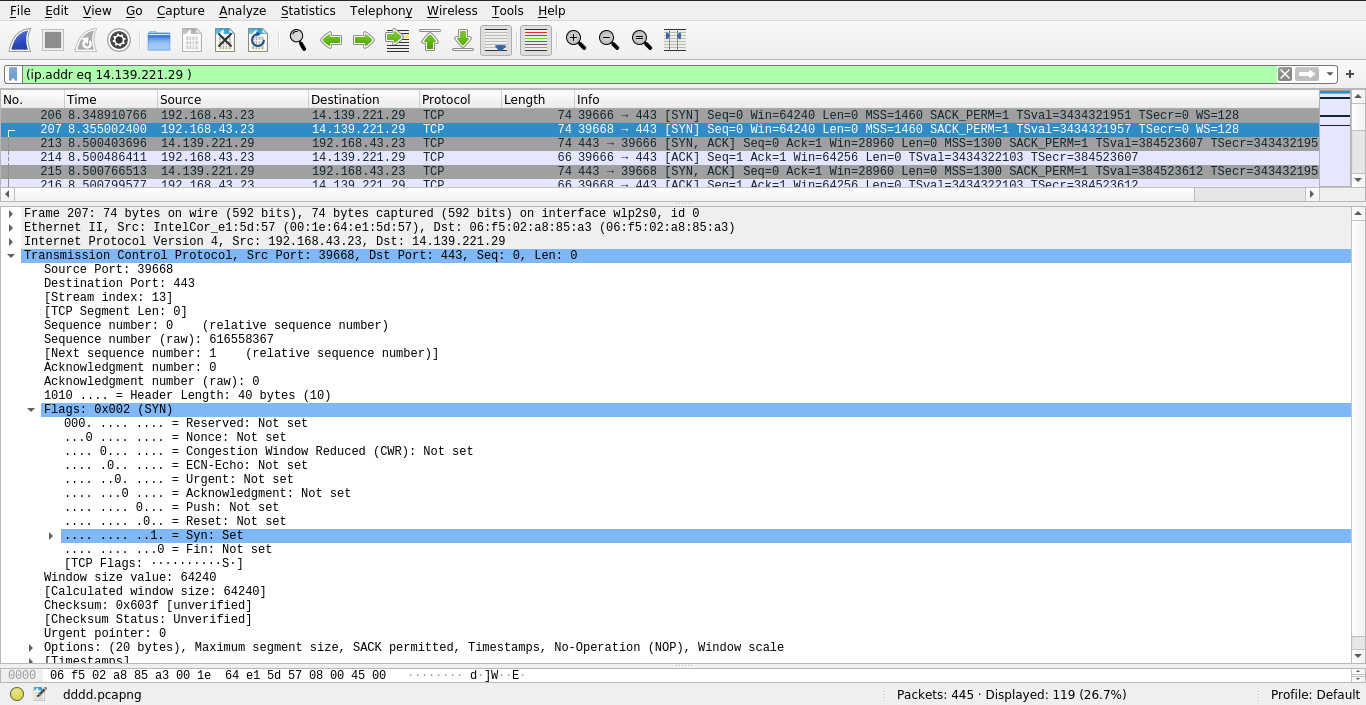
\includegraphics[width=700pt]{Question3D}

\item What is it in the segment that identifies the segment as a SYN segment?

\textbf{Answer.} In the above figure,It is indicated by the Syn flag in the Flags section, which is set to 1.

\item What is the sequence number of the SYN-ACK segment sent by nitdgp.ac.in to the client
computer in reply to the SYN?

\textbf{Answer.} Relative sequence number is 0. And actual sequence number is \textbf{1598426480}. The sequence number	of the TCP SYN segment is 0	since it is used to initate	the	TCP	connection between the client computer and	nitdgp.ac.in.

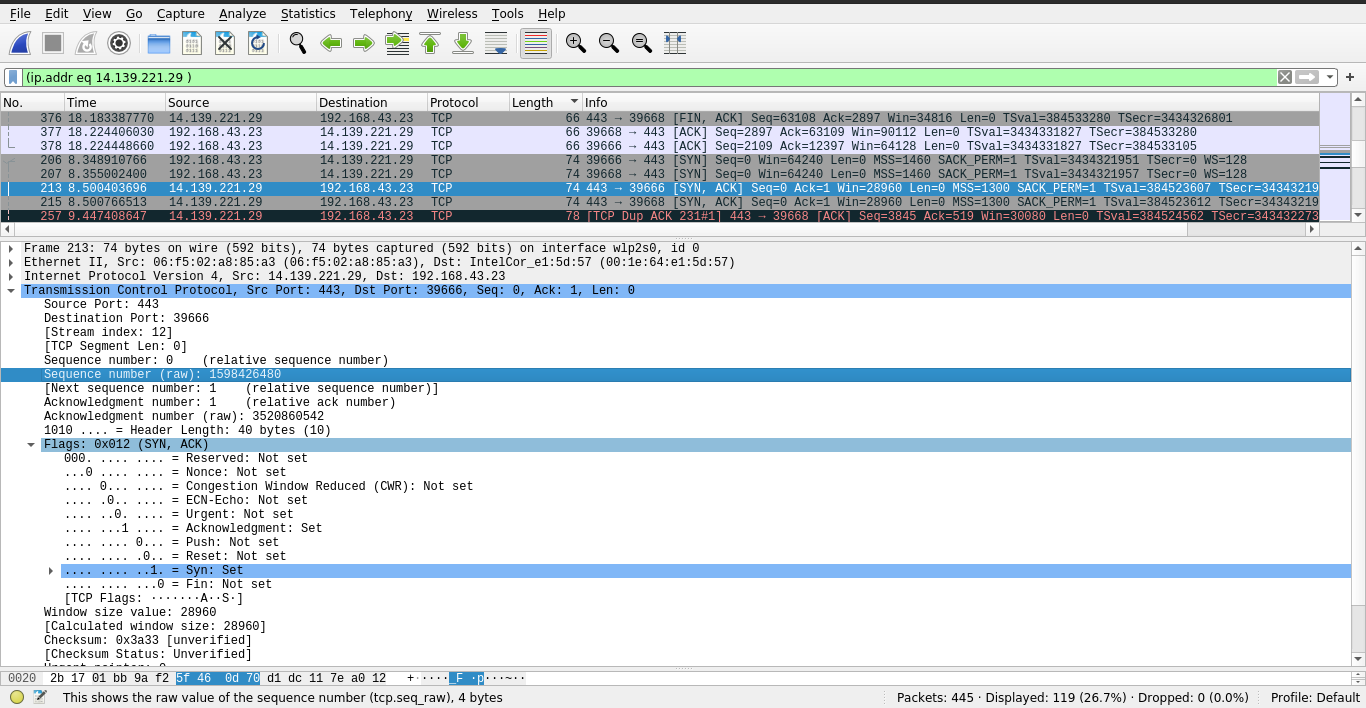
\includegraphics[width=700pt]{Question3F}

\item What is the value of the Acknowledgement field in the SYN-ACK segment?

\textbf{Answer.} According to the above figure, the value of the acknowledgement field in the SYNACK segment is 1.

\item How did nitdgp.ac.in determine that value?

\textbf{Answer.} According to the above figure, the value of the ACK acknowledgement field in the SYNACK segment is determined by the server nitdgp.ac.in. The server adds 1 to the initial sequence number of SYN segment from teh client computer. For this case, the initial sequence number of SYN segment from the client computer is 0, thus the value of the ACK acknowledgement field in the SYNACK segment is 1.

\item What is it in the segment that identifies the segment as a SYN-ACK segment?

\textbf{Answer.} A segment will be identified as a SYNACK segment if both SYN flag and Acknowledgement in the segment are set to 1.

\end{enumerate}
\end{enumerate}

\end{document}
